% State space diagram of the linear growth curve model (vignette lin-growth).
\documentclass[tikz, border = 6pt]{standalone}
\usepackage{amsmath}
\usepackage{bm}
\usetikzlibrary{arrows.meta, positioning, calc}
\tikzset{
  lat/.style = {circle, draw, thick, minimum size = 13mm, inner sep = 0pt},
  obs/.style = {rectangle, draw, thick, minimum size = 11mm, inner sep = 1pt},
  noise/.style = {circle, draw, minimum size = 8mm, inner sep = 0pt},
  reg/.style = {-{Stealth[length = 2.5mm]}, thick},
  lab/.style = {font = \footnotesize, fill = white, inner sep = 1pt},
  mat/.style = {font = \small, inner sep = 2pt, align = left},
  dots/.style = {font = \Large}
}
\begin{document}
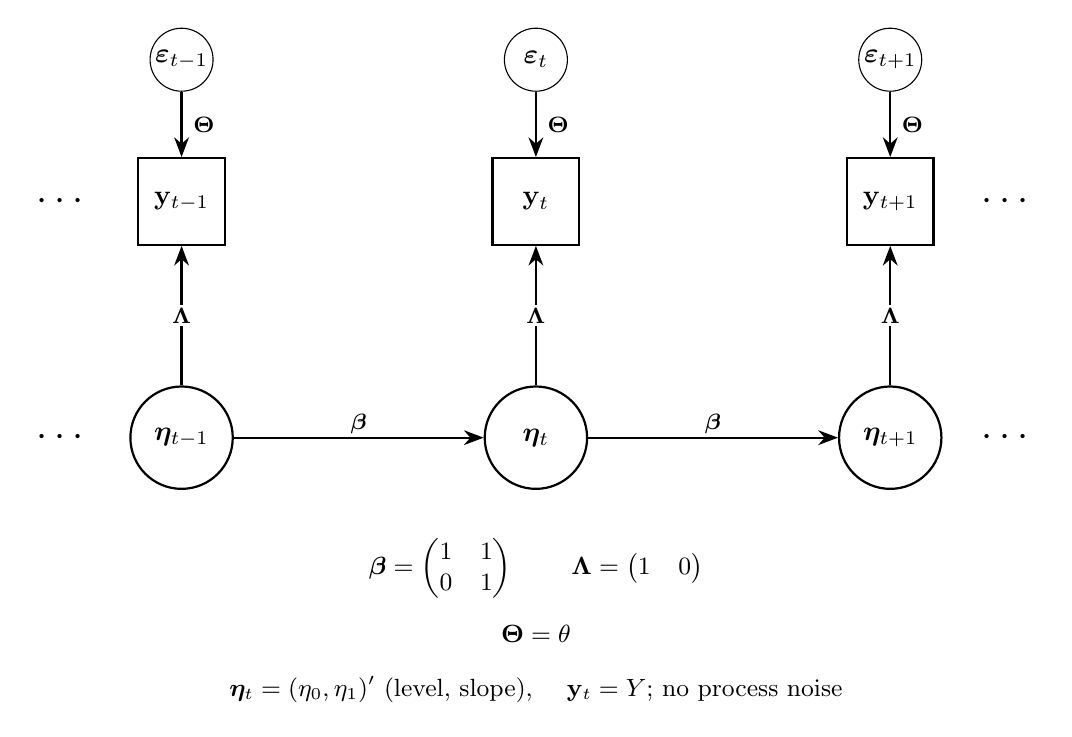
\begin{tikzpicture}
  % occasions
  \node[lat] (e0) at (0, 0) {$\bm{\eta}_{t - 1}$};
  \node[obs] (y0) at (0, 3) {$\mathbf{y}_{t - 1}$};
  \draw[reg] (e0) -- node[lab] {$\bm{\Lambda}$} (y0);
  \node[noise] (u0) at (0, 4.8) {$\bm{\varepsilon}_{t - 1}$};
  \draw[reg] (u0) -- node[lab, right = 1mm] {$\bm{\Theta}$} (y0);
  \node[lat] (e1) at (4.5, 0) {$\bm{\eta}_{t}$};
  \node[obs] (y1) at (4.5, 3) {$\mathbf{y}_{t}$};
  \draw[reg] (e1) -- node[lab] {$\bm{\Lambda}$} (y1);
  \node[noise] (u1) at (4.5, 4.8) {$\bm{\varepsilon}_{t}$};
  \draw[reg] (u1) -- node[lab, right = 1mm] {$\bm{\Theta}$} (y1);
  \node[lat] (e2) at (9.0, 0) {$\bm{\eta}_{t + 1}$};
  \node[obs] (y2) at (9.0, 3) {$\mathbf{y}_{t + 1}$};
  \draw[reg] (e2) -- node[lab] {$\bm{\Lambda}$} (y2);
  \node[noise] (u2) at (9.0, 4.8) {$\bm{\varepsilon}_{t + 1}$};
  \draw[reg] (u2) -- node[lab, right = 1mm] {$\bm{\Theta}$} (y2);
  % transitions
  \draw[reg] (e0) -- node[lab, above] {$\bm{\beta}$} (e1);
  \draw[reg] (e1) -- node[lab, above] {$\bm{\beta}$} (e2);
  \foreach \r in {0, 3} {
    \node[dots] at (-1.5, \r) {$\cdots$};
    \node[dots] at (10.5, \r) {$\cdots$};
  }
  % matrices
  \node[mat, align = center, below] at (4.5, -1.2) {$\bm{\beta} = \begin{pmatrix} 1 & 1 \\ 0 & 1 \end{pmatrix}$ \qquad $\bm{\Lambda} = \begin{pmatrix} 1 & 0 \end{pmatrix}$ \\[3mm] $\bm{\Theta} = \theta$ \\[3mm] $\bm{\eta}_{t} = \left( \eta_{0}, \eta_{1} \right)^{\prime}$ (level, slope), \quad $\mathbf{y}_{t} = Y$; no process noise};
\end{tikzpicture}
\end{document}
